\chapter{Cinética compleja: cadenas, enzimas y oscilaciones}\label{ch:b3:complex-kinetics}

Un vaso de precipitados con una disolución agitada se vuelve incoloro, luego ámbar, luego azul, luego
de nuevo incoloro, y sigue haciéndolo durante muchos minutos; vertida en una placa, la
misma mezcla dibuja espirales que giran y avanzan. Cuando Boris Belousov
describió una reacción así en 1951, su manuscrito fue rechazado: un sistema
químico, pensó el evaluador, no puede ir y volver, ya que debe descender
hacia el equilibrio. Desciende, en efecto; solo que no lo hace en línea
recta. Este capítulo trata los mecanismos de muchas etapas cuyos intermedios
se regeneran: las \omterm{def:b3:complex-kinetics:chain}{reacciones en cadena} y las explosiones, las moléculas que necesitan
colisiones para romperse por sí solas, las \omterm{def:b3:complex-kinetics:enzyme}{enzimas} y las \omterm{def:b3:complex-kinetics:oscillating}{reacciones oscilantes}, junto con
los métodos que siguen reacciones demasiado rápidas para mezclarlas a mano.

\begin{recall}
El volumen del primer año definió un mecanismo de reacción como una secuencia de etapas
elementales, la etapa determinante de la velocidad, las aproximaciones del preequilibrio y del estado
estacionario, y los catalizadores. El volumen del segundo año dio nombre a las etapas de una cadena
radicalaria (iniciación, propagación, terminación), a los iniciadores radicalarios y a la
longitud de cadena cinética de una polimerización, y ajustó rectas por mínimos cuadrados.
El \cref{ch:b3:rate-theories} dio la \omterm{def:b3:rate-theories:tst}{teoría del estado de transición} y el límite de difusión,
de unos \qty{e10}{L.mol^{-1}.s^{-1}}.
\end{recall}

\section{Reacciones en cadena}

\begin{definition}[Reacción en cadena, portador de cadena]\label{def:b3:complex-kinetics:chain}
Una \emph{reacción en cadena}\index{reaccion en cadena@reacción en cadena} es una reacción en la que unos intermedios
reactivos, los \emph{portadores de cadena}\index{portador de cadena}, se regeneran mediante
un ciclo de etapas de propagación, de modo que un solo suceso de iniciación transforma muchas
moléculas de reactivo.
\end{definition}

Bodenstein midió en 1906 la velocidad de $\ce{H2 + Br2 -> 2 HBr}$ y encontró una ley que
ninguna etapa única podía producir: la velocidad crece como $[\ce{Br2}]^{1/2}$ y disminuye a medida que se acumula
el HBr. El mecanismo se escribió en 1919:
\begin{center}
\begin{tabular}{lll}
iniciación & $\ce{Br2 -> 2 Br}$ & $k_1$ \\
propagación & $\ce{Br + H2 -> HBr + H}$ & $k_2$ \\
propagación & $\ce{H + Br2 -> HBr + Br}$ & $k_3$ \\
inhibición & $\ce{H + HBr -> H2 + Br}$ & $k_4$ \\
terminación & $\ce{2 Br -> Br2}$ & $k_{-1}$
\end{tabular}
\end{center}
(las colisiones con un tercer cuerpo M, que aportan y retiran energía en las etapas de
iniciación y de terminación, quedan implícitas).

\begin{theorem}[La ley de velocidad hidrógeno--bromo]\label{thm:b3:complex-kinetics:hbr}
Con la aproximación del estado estacionario para Br y para H, la velocidad $v = \frac12\,\dd[\ce{HBr}]/\dd t$
del mecanismo es
\[
  v = \frac{k[\ce{H2}][\ce{Br2}]^{1/2}}{1 + k'[\ce{HBr}]/[\ce{Br2}]},
  \qquad k = k_2\Bigl(\frac{k_1}{k_{-1}}\Bigr)^{1/2},\ k' = \frac{k_4}{k_3}.
\]
\end{theorem}

\begin{proof}
Estado estacionario para H: $k_2[\ce{Br}][\ce{H2}] = k_3[\ce{H}][\ce{Br2}] + k_4[\ce{H}][\ce{HBr}]$. Estado estacionario para Br:
$2k_1[\ce{Br2}] - k_2[\ce{Br}][\ce{H2}] + k_3[\ce{H}][\ce{Br2}] + k_4[\ce{H}][\ce{HBr}] - 2k_{-1}[\ce{Br}]^2 = 0$. Sumando las dos
ecuaciones, los términos de propagación se cancelan: $k_1[\ce{Br2}] = k_{-1}[\ce{Br}]^2$, luego $[\ce{Br}] =
(k_1/k_{-1})^{1/2}[\ce{Br2}]^{1/2}$. Entonces $[\ce{H}] = k_2[\ce{Br}][\ce{H2}]/(k_3[\ce{Br2}] + k_4[\ce{HBr}])$ y
\[
  \frac{\dd[\ce{HBr}]}{\dd t} = k_2[\ce{Br}][\ce{H2}] + k_3[\ce{H}][\ce{Br2}] - k_4[\ce{H}][\ce{HBr}] = 2k_3[\ce{H}][\ce{Br2}]
  = \frac{2k_2[\ce{Br}][\ce{H2}]}{1 + (k_4/k_3)[\ce{HBr}]/[\ce{Br2}]},
\]
usando la primera ecuación; sustituyendo $[\ce{Br}]$ se obtiene el resultado.
\end{proof}

\begin{omfigure}
\begin{tikzpicture}[font=\small, >=Stealth]
  \node[draw, circle, minimum size=9mm, omDef, thick] (br) at (0,0) {Br};
  \node[draw, circle, minimum size=9mm, omThm, thick] (h) at (4,0) {H};
  \draw[->, thick] (br) to[bend left=35] node[midway, above, align=center] {$+\,\ce{H2}$\\ $\to$ HBr} (h);
  \draw[->, thick] (h) to[bend left=35] node[midway, below, align=center] {$+\,\ce{Br2}$\\ $\to$ HBr} (br);
  \draw[->, thick, black!60] (-2.4,0) -- (br) node[pos=0, left, align=right] {iniciación\\ $\ce{Br2 -> 2 Br}$};
  \draw[->, thick, black!60] (br) -- (0,-2.0) node[below, align=center] {terminación\\ $\ce{2 Br -> Br2}$};
  \draw[->, thick, black!60, dashed] (h) -- (6.2,-1.2) node[below, align=center] {inhibición\\ $\ce{H + HBr -> H2 + Br}$};
\end{tikzpicture}

{\small El ciclo de propagación de la cadena hidrógeno--bromo: cada vuelta consume
un \ce{H2} y un \ce{Br2}, forma dos HBr y devuelve el átomo de bromo que la
inició. La iniciación alimenta el ciclo con portadores y la terminación los elimina;
la etapa de inhibición convierte de nuevo un átomo H en Br a costa de un HBr ya
formado.}
\end{omfigure}

\begin{omfigure}
\begin{tikzpicture}
\begin{axis}[name=ca, width=0.47\linewidth, height=5.2cm, xmin=0, xmax=800, ymin=0, ymax=1,
  axis lines=left, xlabel={$t$ (reducido)}, ylabel={$[\ce{HBr}]/2[\ce{H2}]_0$},
  tick label style={font=\small}, label style={font=\small}]
\addplot[omDef, thick] table[x=t, y expr=\thisrow{HBr}/2] {figdata/out/bachelor-3-chain-kinetics.dat};
\end{axis}
\begin{axis}[at={(ca.east)}, anchor=west, xshift=1.4cm, width=0.47\linewidth, height=5.2cm,
  xmin=0, xmax=60, ymin=0, ymax=2.2, axis lines=left, xlabel={$t$ (reducido)},
  ylabel={velocidad $\times 10^3$}, tick label style={font=\small}, label style={font=\small},
  legend style={font=\scriptsize, draw=none, at={(0.97,0.03)}, anchor=south east},
  legend cell align=left]
\addplot[omDef, thick] table[x=t, y expr=1000*\thisrow{v}] {figdata/out/bachelor-3-chain-kinetics.dat};
\addplot[omThm, thick, dashed] table[x=t, y expr=1000*\thisrow{vss}] {figdata/out/bachelor-3-chain-kinetics.dat};
\legend{mecanismo completo, ley del estado estacionario}
\end{axis}
\end{tikzpicture}

{\small El mecanismo hidrógeno--bromo integrado etapa por etapa (constantes de velocidad
modelo, unidades reducidas, $k' = 0.1$): conversión en función del tiempo (izquierda), y la velocidad
$\frac12\dd[\ce{HBr}]/\dd t$ del mecanismo completo comparada con la ley del estado estacionario (derecha).
Tras un periodo de inducción, durante el cual se acumulan los átomos de bromo, ambas
coinciden con una precisión mejor que el 1\,\%.}
\end{omfigure}

\begin{method}[La ley de velocidad de un mecanismo en cadena]\label{met:b3:complex-kinetics:steady-state-chain}
\begin{enumerate}
  \item Escribir una ecuación de estado estacionario para cada \omterm{def:b3:complex-kinetics:chain}{portador de cadena}.
  \item Sumarlas: las etapas de propagación, que solo cambian un portador por
        otro, se cancelan, y queda la iniciación igual a la terminación; esto da la
        concentración de portadores.
  \item Usar la ecuación de un portador para expresar los demás.
  \item Escribir la velocidad de formación de un producto a partir de las etapas de propagación.
\end{enumerate}
\end{method}

El número de ciclos de propagación por suceso de iniciación, aquí $v/k_1[\ce{Br2}]$, es la
longitud de cadena cinética del volumen del segundo año; para la reacción hidrógeno--bromo
es del orden de $10^3$ a $10^6$ según las condiciones. La inhibición por
el producto explica por qué la velocidad disminuye más deprisa de lo que se consumen los reactivos.

\section{Cadenas ramificadas y explosiones}

\begin{definition}[Ramificación de cadena, límites de explosión]\label{def:b3:complex-kinetics:branching}
La \emph{ramificación de cadena}\index{ramificacion de cadena@ramificación de cadena} es una etapa de propagación que produce
más \omterm{def:b3:complex-kinetics:chain}{portadores de cadena} de los que consume, como $\ce{H + O2 -> OH + O}$, que convierte un
portador en dos. Los \emph{límites de explosión}\index{limites de explosion@límites de explosión} de una mezcla
son las presiones, a una temperatura dada, a las que su reacción lenta se convierte
en una explosión.
\end{definition}

\begin{proposition}[Criterio de ramificación]\label{prop:b3:complex-kinetics:branching}
Sean portadores creados a la velocidad $v_i$, que se multiplican por ramificación con la constante
de velocidad $f$ y desaparecen por terminación con la constante de velocidad $g$:
$\dd n/\dd t = v_i + (f - g)n$. Si $f < g$, $n$ tiende al valor estacionario $v_i/(g - f)$; si
$f > g$, $n$ crece exponencialmente y la reacción explota.
\end{proposition}

\begin{proof}
La ecuación lineal tiene la solución $n(t) = \frac{v_i}{g - f}\bigl(1 - \eu^{-(g - f)t}\bigr)$, que
tiende a $v_i/(g - f)$ cuando $g > f$; cuando $f > g$, el exponente es positivo y $n$
crece como $\eu^{(f - g)t}$ sin límite (hasta que se agotan los reactivos).
\end{proof}

Para las mezclas de hidrógeno y oxígeno a unos cientos de grados, $f$ crece con la
presión (es proporcional a $[\ce{O2}]$), la terminación en las paredes del
recipiente es rápida a baja presión (los radicales difunden fácilmente hasta ellas), y la
terminación por colisiones de tres cuerpos ($\ce{H + O2 + M -> HO2 + M}$) crece como el cuadrado
de la presión. La ramificación gana entre un primer límite, fijado por las paredes, y un
segundo límite, fijado por la terminación de tres cuerpos; a presión todavía mayor aparece un tercer
límite, en el que el calor liberado ya no puede escapar. Este último es una
explosión térmica, impulsada por el crecimiento exponencial de la velocidad con la
temperatura más que por la ramificación; la mayoría de las explosiones industriales son de ese
tipo.

\section{Reacciones unimoleculares}

Una molécula como el ciclopropano se isomeriza sola, con una cinética de primer orden a
presiones ordinarias; sin embargo, a baja presión la constante de velocidad disminuye. La energía
necesaria procede de las colisiones.

\begin{definition}[Mecanismo de Lindemann, región de caída]\label{def:b3:complex-kinetics:lindemann}
El \emph{mecanismo de Lindemann}\index{mecanismo de Lindemann} de una reacción
unimolecular es la secuencia $\mathrm{A + M \rightleftharpoons A^* + M}$ ($k_1$, $k_{-1}$), activación y
desactivación por colisión con cualquier molécula M, seguida de $\mathrm{A^* \to P}$ ($k_2$). La
\emph{región de caída}\index{region de caida@región de caída} es el intervalo de presiones en el que la
constante de velocidad de primer orden observada cae desde su valor de alta presión hacia un
comportamiento de segundo orden.
\end{definition}

\begin{theorem}[Constante de velocidad de Lindemann]\label{thm:b3:complex-kinetics:lindemann}
Con la aproximación del estado estacionario para $\mathrm{A^*}$, $v = k_{\mathrm{uni}}[\mathrm A]$ con
\[
  k_{\mathrm{uni}} = \frac{k_1k_2[\mathrm M]}{k_{-1}[\mathrm M] + k_2},
\]
que tiende a $k_\infty = k_1k_2/k_{-1}$ a alta presión (primer orden) y a $k_1[\mathrm M]$ a
baja presión (segundo orden); vale $k_\infty/2$ en $[\mathrm M]_{1/2} = k_2/k_{-1}$.
\end{theorem}

\begin{proof}
$\dd[\mathrm{A^*}]/\dd t = k_1[\mathrm A][\mathrm M] - k_{-1}[\mathrm{A^*}][\mathrm M] - k_2[\mathrm{A^*}] = 0$ da $[\mathrm{A^*}] =
k_1[\mathrm A][\mathrm M]/(k_{-1}[\mathrm M] + k_2)$ y $v = k_2[\mathrm{A^*}]$. Si $k_{-1}[\mathrm M] \gg k_2$, la desactivación
supera a la reacción y $\mathrm{A^*}$ está en preequilibrio: $k_{\mathrm{uni}} \to k_1k_2/k_{-1}$. Si $k_{-1}[\mathrm M]
\ll k_2$, toda molécula activada reacciona y la activación es la etapa determinante:
$k_{\mathrm{uni}} \to k_1[\mathrm M]$.
\end{proof}

\begin{omfigure}
\begin{tikzpicture}
\begin{axis}[width=0.66\linewidth, height=5.4cm, xmode=log, ymode=log, xmin=1e-10, xmax=1e-2,
  ymin=1e-8, ymax=4e-3, axis lines=left, xlabel={$[\mathrm M]$ / \unit{mol.L^{-1}}},
  ylabel={$k_{\mathrm{uni}}$ / \unit{s^{-1}}}, tick label style={font=\small}, label style={font=\small}]
\addplot[black!40, dashed] table[x=M, y=low] {figdata/out/bachelor-3-lindemann.dat};
\addplot[black!40, dashed] table[x=M, y=high] {figdata/out/bachelor-3-lindemann.dat};
\addplot[omDef, very thick] table[x=M, y=k] {figdata/out/bachelor-3-lindemann.dat};
\node[font=\scriptsize, anchor=south, rotate=39] at (axis cs:4e-9,2.5e-5) {$k_1[\mathrm M]$};
\node[font=\scriptsize, anchor=south] at (axis cs:3e-4,1e-3) {$k_\infty$};
\draw[black!50, densely dotted] (axis cs:1e-6,1e-8) -- (axis cs:1e-6,5e-4);
\node[font=\scriptsize, anchor=north west] at (axis cs:1.2e-6,2e-7) {$[\mathrm M]_{1/2}$};
\end{axis}
\end{tikzpicture}

{\small La curva de caída de Lindemann (constantes modelo): primer orden con la
constante límite $k_\infty$ a alta presión, segundo orden ($k_1[\mathrm M]$) a baja presión,
y la mitad de $k_\infty$ en $[\mathrm M]_{1/2} = k_2/k_{-1}$. Las curvas de caída reales son más anchas: la constante
de velocidad $k_2$ de una molécula energizada crece con su energía.}
\end{omfigure}

\section{Cinética enzimática}

\begin{definition}[Enzima, sitio activo, complejo enzima--sustrato]\label{def:b3:complex-kinetics:enzyme}
Una \emph{enzima}\index{enzima} es un catalizador biológico, casi siempre una proteína,
que acelera una reacción específica de su sustrato. El \emph{sitio
activo}\index{sitio activo} es la cavidad de la enzima donde el sustrato se une
y reacciona; la especie unida es el \emph{complejo
enzima--sustrato}\index{complejo enzima--sustrato} ES.
\end{definition}

\begin{definition}[Constante de Michaelis, velocidad máxima, constantes catalítica y de especificidad]\label{def:b3:complex-kinetics:michaelis}
Para el mecanismo $\mathrm{E + S \rightleftharpoons ES \to E + P}$ ($k_1$, $k_{-1}$, $k_2$) con una concentración total de \omterm{def:b3:complex-kinetics:enzyme}{enzima}
$[\mathrm E]_0$, la \emph{constante catalítica}\index{constante catalitica@constante catalítica} es $k_{\mathrm{cat}} = k_2$, la
\emph{velocidad máxima}\index{velocidad maxima@velocidad máxima} es $V_{\max} = k_{\mathrm{cat}}[\mathrm E]_0$, la \emph{constante de Michaelis}
\index{constante de Michaelis} es $K_M = (k_{-1} + k_2)/k_1$, y la \emph{constante de especificidad}
\index{constante de especificidad} es $k_{\mathrm{cat}}/K_M$.
\end{definition}

\begin{theorem}[Ecuación de Michaelis--Menten]\label{thm:b3:complex-kinetics:michaelis-menten}
Cuando $[\mathrm S] \gg [\mathrm E]_0$ y ES está en estado estacionario, la velocidad inicial de formación
del producto es
\[
  v = \frac{V_{\max}[\mathrm S]}{K_M + [\mathrm S]} .
\]
Este enunciado es la \emph{ecuación de Michaelis--Menten}\index{ecuacion de Michaelis--Menten@ecuación de Michaelis--Menten}.
\end{theorem}

\begin{proof}
Estado estacionario: $k_1[\mathrm E][\mathrm S] = (k_{-1} + k_2)[\mathrm{ES}]$, y $[\mathrm E] = [\mathrm E]_0 - [\mathrm{ES}]$ (el sustrato
libre es prácticamente todo el sustrato, ya que $[\mathrm S] \gg [\mathrm E]_0$). Por tanto, $[\mathrm{ES}]
= [\mathrm E]_0[\mathrm S]/(K_M + [\mathrm S])$ y $v = k_2[\mathrm{ES}]$.
\end{proof}

\begin{remark}
Michaelis y Menten (1913) supusieron en cambio un preequilibrio rápido entre E, S y
ES; se obtiene la misma ecuación con $K_M$ sustituida por la constante de disociación
$k_{-1}/k_1$, el límite de $K_M$ cuando $k_2 \ll k_{-1}$. La \omterm{def:b3:complex-kinetics:michaelis}{constante catalítica} es lo que
los bioquímicos llaman número de recambio de la \omterm{def:b3:complex-kinetics:enzyme}{enzima}: el número de moléculas de sustrato
que un \omterm{def:b3:complex-kinetics:enzyme}{sitio activo} transforma por segundo cuando está saturado.
\end{remark}

En $[\mathrm S] = K_M$, la velocidad es $V_{\max}/2$; para $[\mathrm S] \ll K_M$ vale $(k_{\mathrm{cat}}/K_M)[\mathrm E]_0[\mathrm S]$: la
\omterm{def:b3:complex-kinetics:michaelis}{constante de especificidad} es la constante de velocidad de segundo orden de la \omterm{def:b3:complex-kinetics:enzyme}{enzima} libre con
su sustrato, y no puede superar la velocidad a la que se encuentran, el
límite de difusión del \cref{ch:b3:rate-theories}. Unas pocas \omterm{def:b3:complex-kinetics:enzyme}{enzimas} se acercan a él; la \omterm{def:b3:complex-kinetics:enzyme}{enzima}
``media'', en un estudio de varios miles, tiene una $k_{\mathrm{cat}}/K_M$ de unos
$10^5$~\unit{L.mol^{-1}.s^{-1}}, unos cuatro órdenes de magnitud por debajo.

\begin{proposition}[Forma de Lineweaver--Burk]\label{prop:b3:complex-kinetics:lineweaver}
La \omterm{thm:b3:complex-kinetics:michaelis-menten}{ecuación de Michaelis--Menten} equivale a
\[
  \frac1v = \frac{1}{V_{\max}} + \frac{K_M}{V_{\max}}\,\frac{1}{[\mathrm S]},
\]
una recta de $1/v$ en función de $1/[\mathrm S]$, de ordenada en el origen $1/V_{\max}$, pendiente $K_M/V_{\max}$ e
intersección $-1/K_M$ con el eje $1/[\mathrm S]$.
\end{proposition}

\begin{proof}
Se invierte: $1/v = (K_M + [\mathrm S])/(V_{\max}[\mathrm S])$. Para $1/v = 0$, $1/[\mathrm S] = -1/K_M$.
\end{proof}

\begin{method}[$K_M$ y $V_{\max}$ por mínimos cuadrados no lineales]\label{met:b3:complex-kinetics:mm-fit}
\begin{enumerate}
  \item Medir velocidades iniciales a concentraciones de sustrato repartidas desde unos
        $K_M/5$ hasta $10K_M$.
  \item Ajustar directamente $v = V_{\max}[\mathrm S]/(K_M + [\mathrm S])$ minimizando $\sum(v_i - v(\mathrm S_i))^2$ (de forma iterativa,
        partiendo de los valores de una recta de Lineweaver--Burk); los errores
        típicos se obtienen de los residuos y de la sensibilidad de $v$ a cada
        parámetro.
  \item Usar la gráfica de Lineweaver--Burk solo para ver el patrón: invertir velocidades
        pequeñas amplifica sus errores, de modo que la recta de mínimos cuadrados de $1/v$
        está dominada por los puntos menos precisos, y sus parámetros están
        sesgados.
\end{enumerate}
\end{method}

\begin{definition}[Inhibición]\label{def:b3:complex-kinetics:inhibition}
Un inhibidor I se une a la \omterm{def:b3:complex-kinetics:enzyme}{enzima} de forma reversible. En la \emph{inhibición
competitiva}\index{inhibicion competitiva@inhibición competitiva} solo se une a la \omterm{def:b3:complex-kinetics:enzyme}{enzima} libre, en el
\omterm{def:b3:complex-kinetics:enzyme}{sitio activo}, con la \emph{constante de inhibición}\index{constante de inhibicion@constante de inhibición} $K_i$
(constante de disociación de EI); en la \emph{inhibición acompetitiva}\index{inhibicion acompetitiva@inhibición acompetitiva}
solo se une a ES, con la constante $K_i'$; en la \emph{inhibición
mixta}\index{inhibicion mixta@inhibición mixta} se une a ambas.
\end{definition}

\begin{proposition}[Leyes de velocidad con inhibición]\label{prop:b3:complex-kinetics:inhibition-laws}
Con $\alpha = 1 + [\mathrm I]/K_i$ y $\alpha' = 1 + [\mathrm I]/K_i'$, la velocidad conserva la
forma de Michaelis--Menten $v = V^{\mathrm{app}}[\mathrm S]/(K_M^{\mathrm{app}} + [\mathrm S])$ con: competitiva,
$K_M^{\mathrm{app}} = \alpha K_M$, $V^{\mathrm{app}} = V_{\max}$; acompetitiva, $K_M^{\mathrm{app}} = K_M/\alpha'$, $V^{\mathrm{app}} =
V_{\max}/\alpha'$; mixta, $K_M^{\mathrm{app}} = \alpha K_M/\alpha'$, $V^{\mathrm{app}} = V_{\max}/\alpha'$.
\end{proposition}

\begin{proof}
Caso mixto (los demás son sus límites $K_i' \to \infty$ y $K_i \to \infty$): la \omterm{def:b3:complex-kinetics:enzyme}{enzima} se
reparte entre E, EI, ES y ESI con $[\mathrm{EI}] = [\mathrm E][\mathrm I]/K_i$, $[\mathrm{ESI}] = [\mathrm{ES}][\mathrm I]/K_i'$
y el estado estacionario $[\mathrm E][\mathrm S] = K_M[\mathrm{ES}]$. Así, $[\mathrm E]_0 = [\mathrm E]\alpha + [\mathrm{ES}]\alpha' =
[\mathrm{ES}](\alpha K_M/[\mathrm S] + \alpha')$ y $v = k_2[\mathrm{ES}] = V_{\max}[\mathrm S]/(\alpha K_M + \alpha'[\mathrm S])$; dividiendo numerador
y denominador por $\alpha'$ se obtiene la forma enunciada.
\end{proof}

\begin{method}[Reconocer el tipo de inhibición]\label{met:b3:complex-kinetics:inhibition-type}
\begin{enumerate}
  \item Medir $v([\mathrm S])$ a varias concentraciones de inhibidor y trazar las
        rectas de Lineweaver--Burk.
  \item Rectas que se cortan sobre el eje $1/v$ (misma $V_{\max}$): competitiva; un gran exceso
        de sustrato vence al inhibidor.
  \item Rectas paralelas (pendiente $K_M/V_{\max}$ sin cambio): acompetitiva.
  \item Rectas que se cortan a la izquierda del eje $1/v$: mixta.
  \item Obtener $K_i$ ajustando las constantes aparentes en función de $[\mathrm I]$: para un
        inhibidor competitivo, $K_M^{\mathrm{app}} = K_M + (K_M/K_i)[\mathrm I]$, una recta.
\end{enumerate}
\end{method}

\begin{omfigure}
\begin{tikzpicture}
\begin{axis}[name=mv, width=0.47\linewidth, height=5.4cm, xmin=0, xmax=8, ymin=0, ymax=0.55,
  axis lines=left, xlabel={$[\mathrm S]$ / mM}, ylabel={$v$ / \unit{\micro M.s^{-1}}},
  tick label style={font=\small}, label style={font=\small},
  legend style={font=\scriptsize, draw=none, fill=white, fill opacity=0.85, text opacity=1,
  at={(0.97,0.03)}, anchor=south east}, legend cell align=left]
\addplot[black, thick] table[x=S, y=none] {figdata/out/bachelor-3-michaelis-menten-model.dat};
\addplot[omDef, thick] table[x=S, y=comp] {figdata/out/bachelor-3-michaelis-menten-model.dat};
\addplot[omThm, thick] table[x=S, y=uncomp] {figdata/out/bachelor-3-michaelis-menten-model.dat};
\draw[black!40, densely dotted] (axis cs:0,0.25) -- (axis cs:0.8,0.25) -- (axis cs:0.8,0);
\node[font=\scriptsize, anchor=north west] at (axis cs:0.85,0.12) {$K_M$};
\legend{sin inhibidor, competitiva, acompetitiva}
\end{axis}
\begin{axis}[at={(mv.east)}, anchor=west, xshift=1.5cm, width=0.47\linewidth, height=5.4cm,
  xmin=-2.5, xmax=3.5, ymin=0, ymax=12, axis x line=middle, axis y line=middle,
  tick label style={font=\small}, xtick={-2,-1,1,2,3}]
\node[font=\small, anchor=south east] at (axis cs:3.5,0.3) {$1/[\mathrm S]$};
\node[font=\small, anchor=north west] at (axis cs:0.12,12) {$1/v$};
\addplot[black, thick, domain=-1.25:3.5] {1.6*x + 2};
\addplot[omDef, thick, domain=-0.4167:3.5] {4.8*x + 2};
\addplot[omThm, thick, domain=-2.5:3.5] {1.6*x + 4};
\end{axis}
\end{tikzpicture}

{\small Cinética de Michaelis--Menten con $K_M = \qty{0.80}{mM}$ y $V_{\max} = \qty{0.50}{\micro M.s^{-1}}$
(modelo): sin inhibidor (negro), con un inhibidor competitivo a $[\mathrm I] = 2K_i$ (azul,
$K_M$ triplicada, misma $V_{\max}$) y con uno acompetitivo a $[\mathrm I] = K_i'$ (rojo, $K_M$ y
$V_{\max}$ divididas por dos). Derecha: las rectas de Lineweaver--Burk; la recta competitiva corta
a la no inhibida sobre el eje $1/v$, y la acompetitiva es paralela a ella
($1/[\mathrm S]$ en \unit{mM^{-1}}, $1/v$ en \unit{s.\micro M^{-1}}).}
\end{omfigure}

\section{Autocatálisis, oscilaciones y reacciones rápidas}

\begin{definition}[Reacción autocatalítica]\label{def:b3:complex-kinetics:autocatalysis}
Una \emph{reacción autocatalítica}\index{reaccion autocatalitica@reacción autocatalítica} es aquella en la que un
producto cataliza su propia formación, como en $\mathrm{A + X \to 2\,X}$.
\end{definition}

\begin{proposition}[Ley logística]\label{prop:b3:complex-kinetics:logistic}
Para $\mathrm{A + X \to 2\,X}$ con constante de velocidad $k$ y concentraciones iniciales $a_0$ y $x_0$,
con $N = a_0 + x_0$,
\[
  x(t) = \frac{N}{1 + (N/x_0 - 1)\eu^{-kNt}},
\]
una curva en forma de S que alcanza la mitad de su valor final en $t_{1/2} = \ln(N/x_0 - 1)/kN$.
\end{proposition}

\begin{proof}
$\dd x/\dd t = kx(N - x)$, ya que $a = N - x$. Separando variables, $\frac{\dd x}{x(N - x)} = \frac1N\bigl(\frac1x + \frac{1}{N - x}\bigr)\dd x
= k\,\dd t$, luego $\ln\frac{x}{N - x} = kNt + \ln\frac{x_0}{N - x_0}$, que se reordena en la forma enunciada;
$x = N/2$ cuando $(N/x_0 - 1)\eu^{-kNt} = 1$.
\end{proof}

\begin{definition}[Reacción oscilante, ciclo límite]\label{def:b3:complex-kinetics:oscillating}
Una \emph{reacción oscilante}\index{reaccion oscilante@reacción oscilante} es aquella en la que las
concentraciones de los intermedios suben y bajan periódicamente mientras la reacción
global avanza hacia el equilibrio. Un \emph{ciclo límite}\index{ciclo limite@ciclo límite} es
una trayectoria cerrada en el espacio de las concentraciones hacia la que convergen las trayectorias
vecinas, de modo que la oscilación tiene una amplitud independiente
del punto de partida.
\end{definition}

\begin{theorem}[Modelo de Lotka--Volterra]\label{thm:b3:complex-kinetics:lotka-volterra}
Para el esquema autocatalítico $\mathrm{A + X \to 2\,X}$, $\mathrm{X + Y \to 2\,Y}$, $\mathrm{Y \to B}$ con A mantenido
constante, las concentraciones obedecen a $\dot x = x(a - by)$, $\dot y = y(dx - c)$ con constantes
positivas, y la magnitud
\[
  V = dx - c\ln x + by - a\ln y
\]
es constante a lo largo de cada trayectoria: las trayectorias son curvas cerradas en torno
al estado estacionario $(c/d, a/b)$, y las concentraciones oscilan con una
amplitud fijada por el punto de partida.
\end{theorem}

\begin{proof}
$\dot V = (d - c/x)\dot x + (b - a/y)\dot y = (dx - c)(a - by) + (by - a)(dx - c) = 0$. $V$ es una
suma de dos funciones convexas con un único mínimo en $(c/d, a/b)$, de modo que sus curvas
de nivel son curvas cerradas en torno a ese punto; una trayectoria permanece en una de
ellas y, como la velocidad no se anula en ningún otro sitio, la recorre periódicamente.
\end{proof}

Las oscilaciones de Lotka--Volterra son frágiles: cada punto de partida da su
propia órbita, y cualquier perturbación lleva el sistema a otra. Los osciladores químicos
reales tienen un \omterm{def:b3:complex-kinetics:oscillating}{ciclo límite}, que necesita una no linealidad que desestabilice
el estado estacionario.

\begin{proposition}[Inestabilidad del bruselador]\label{prop:b3:complex-kinetics:hopf}
El modelo $\dot X = A - (B + 1)X + X^2Y$, $\dot Y = BX - X^2Y$ (concentraciones reducidas,
$A$ y $B$ mantenidas constantes) tiene un único estado estacionario, $(A, B/A)$, que es
estable si $B < 1 + A^2$ e inestable si $B > 1 + A^2$; el sistema se instala entonces en un
\omterm{def:b3:complex-kinetics:oscillating}{ciclo límite}.
\end{proposition}

\begin{proof}
Anulando ambas derivadas: $BX = X^2Y$ da $XY = B$, y después $A - X = 0$. La
matriz jacobiana en $(A, B/A)$ es
\[
  \begin{pmatrix} -(B + 1) + 2XY & X^2 \\ B - 2XY & -X^2 \end{pmatrix}
  = \begin{pmatrix} B - 1 & A^2 \\ -B & -A^2 \end{pmatrix},
\]
con traza $B - 1 - A^2$ y determinante $A^2 > 0$. Las pequeñas desviaciones evolucionan como
$\eu^{\lambda t}$, con $\lambda$ los \omterm{def:b3:quantum-model-systems:operator}{valores propios}, cuyo producto es el determinante (positivo)
y cuya suma es la traza: ambos tienen parte real negativa cuando la traza es
negativa y parte real positiva cuando es positiva. La existencia del \omterm{def:b3:complex-kinetics:oscillating}{ciclo
límite} para $B > 1 + A^2$ (con las trayectorias confinadas en una región acotada) se
admite.
\end{proof}

\begin{method}[La estabilidad lineal de un estado estacionario]\label{met:b3:complex-kinetics:stability}
\begin{enumerate}
  \item Encontrar el estado estacionario anulando todas las derivadas temporales.
  \item Calcular allí la matriz jacobiana de las derivadas parciales de las velocidades.
  \item Para dos variables: estable si la traza es negativa y el determinante
        positivo; un estado inestable con \omterm{def:b3:quantum-model-systems:operator}{valores propios} complejos
        ($\mathrm{tr}^2 < 4\det$) da oscilaciones crecientes, candidatas a un \omterm{def:b3:complex-kinetics:oscillating}{ciclo límite}.
\end{enumerate}
\end{method}

\begin{omfigure}
\begin{tikzpicture}
\begin{axis}[name=bs, width=0.62\linewidth, height=4.6cm, xmin=0, xmax=40, ymin=0, ymax=5.2,
  axis lines=left, xlabel={$t$ (reducido)}, ylabel={concentración},
  tick label style={font=\small}, label style={font=\small},
  legend style={font=\scriptsize, draw=none, at={(1.03,0.98)}, anchor=north west}]
\addplot[omDef, thick] table[x=t, y=X] {figdata/out/bachelor-3-oscillations-series.dat};
\addplot[omThm, thick] table[x=t, y=Y] {figdata/out/bachelor-3-oscillations-series.dat};
\legend{$X$, $Y$}
\end{axis}
\begin{axis}[name=ph, at={(bs.below south west)}, anchor=north west, yshift=-0.6cm,
  width=0.42\linewidth, height=5.0cm, xmin=0, xmax=4.8, ymin=0, ymax=5.6, axis lines=left,
  xlabel={$X$}, ylabel={$Y$}, tick label style={font=\small}, label style={font=\small},
  title={\small bruselador}]
\addplot[omDef, thin] table[x=X, y=Y] {figdata/out/bachelor-3-oscillations-inner.dat};
\addplot[omThm, thin] table[x=X, y=Y] {figdata/out/bachelor-3-oscillations-outer.dat};
\addplot[only marks, mark=*, mark size=1.5pt] coordinates {(1,3)};
\end{axis}
\begin{axis}[at={(ph.east)}, anchor=west, xshift=1.3cm, width=0.42\linewidth, height=5.0cm,
  xmin=0, xmax=3.2, ymin=0, ymax=3.2, axis lines=left, xlabel={$x$}, ylabel={$y$},
  tick label style={font=\small}, label style={font=\small}, title={\small Lotka--Volterra}]
\addplot[black!70, thick] table[x=x, y=y] {figdata/out/bachelor-3-oscillations-lv1.dat};
\addplot[omDef, thick] table[x=x, y=y] {figdata/out/bachelor-3-oscillations-lv2.dat};
\addplot[omThm, thick] table[x=x, y=y] {figdata/out/bachelor-3-oscillations-lv3.dat};
\addplot[only marks, mark=*, mark size=1.5pt] coordinates {(1,1)};
\end{axis}
\end{tikzpicture}

{\small Arriba: el bruselador ($A = 1$, $B = 3 > 1 + A^2$) se instala en oscilaciones
sostenidas de periodo 7.2 (tiempo reducido). Abajo a la izquierda: dos trayectorias, una
que parte cerca del estado estacionario inestable (punto) y otra muy fuera, se enrollan en
el mismo \omterm{def:b3:complex-kinetics:oscillating}{ciclo límite}. Abajo a la derecha: órbitas de Lotka--Volterra, cada una fijada por su
punto de partida, en torno al estado estacionario (punto).}
\end{omfigure}

La reacción de Belousov--Zhabotinsky, la oxidación del ácido malónico por el bromato
catalizada por el cerio o por el indicador ferroína, recorre un ciclo así: una
producción autocatalítica de \ce{HBrO2} se activa cuando el bromuro cae por debajo de un
umbral, oxida el catalizador (el cambio de color) y se desactiva cuando
el catalizador oxidado regenera el bromuro. Sin agitar, en una capa fina, la
oscilación se propaga en forma de ondas.

\begin{omfigure}
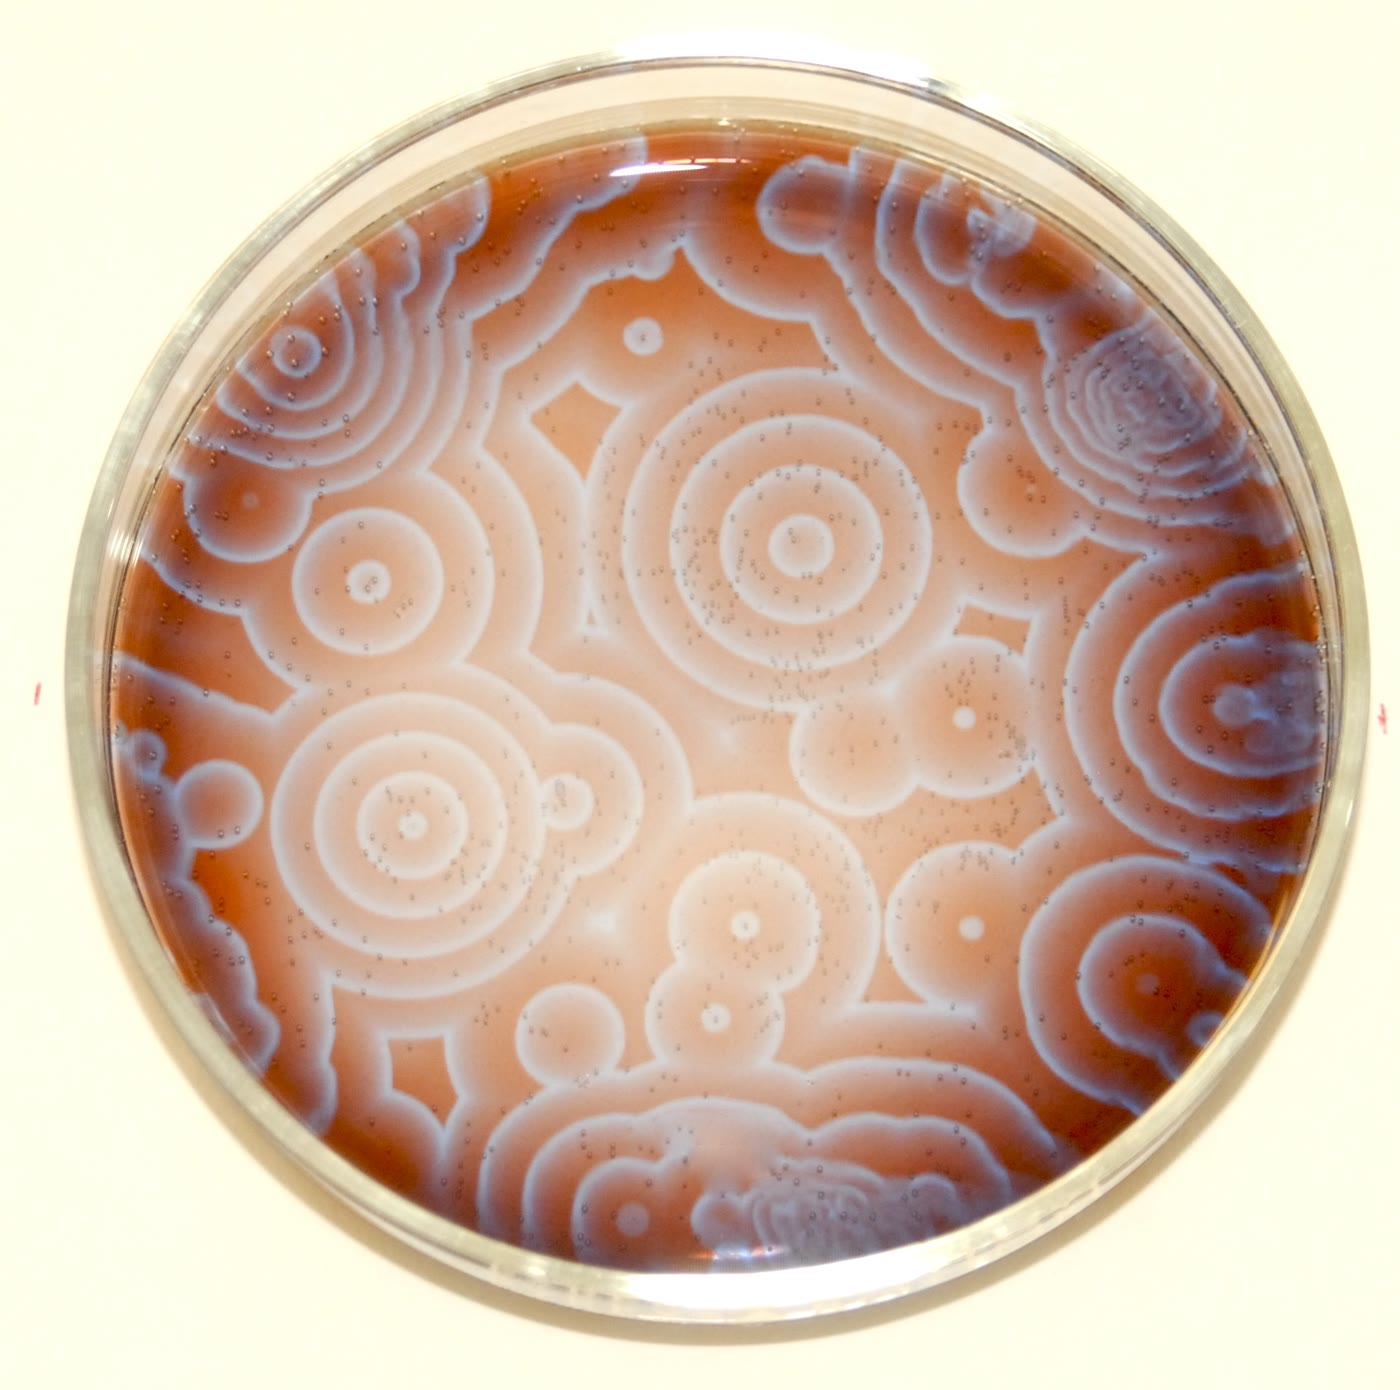
\includegraphics[width=0.48\linewidth]{images/book4/bz-reaction.jpg}

{\small Ondas espirales de la reacción de Belousov--Zhabotinsky en una capa fina de
disolución: cada frente azul es una onda de oxidación del catalizador, que
avanza hacia el medio reducido (rojo) y no puede volver a entrar en la región que acaba de
dejar.}
\end{omfigure}

\begin{definition}[Método de relajación, tiempo de relajación química]\label{def:b3:complex-kinetics:relaxation}
Un \emph{método de relajación}\index{metodo de relajacion@método de relajación} perturba bruscamente un sistema en
equilibrio (mediante un salto de temperatura, de presión o de campo eléctrico)
y sigue su retorno al nuevo equilibrio. Para una perturbación pequeña, la
desviación decae exponencialmente, con el \emph{tiempo de relajación
química}\index{tiempo de relajacion quimica@tiempo de relajación química} $\tau$.
\end{definition}

\begin{proposition}[Tiempo de relajación de una asociación]\label{prop:b3:complex-kinetics:relaxation-time}
Para $\mathrm{A + B \rightleftharpoons C}$ ($k_1$, $k_{-1}$), tras una pequeña perturbación,
\[
  \frac1\tau = k_1([\mathrm A]_e + [\mathrm B]_e) + k_{-1} .
\]
\end{proposition}

\begin{proof}
Se escribe $[\mathrm C] = [\mathrm C]_e + x$, $[\mathrm A] = [\mathrm A]_e - x$, $[\mathrm B] = [\mathrm B]_e - x$. Entonces $\dot x =
k_1([\mathrm A]_e - x)([\mathrm B]_e - x) - k_{-1}([\mathrm C]_e + x)$; los términos sin $x$ se cancelan en el
equilibrio y, despreciando $x^2$: $\dot x = -[k_1([\mathrm A]_e + [\mathrm B]_e) + k_{-1}]x$.
\end{proof}

Medir $\tau$ a varias concentraciones da una recta de $1/\tau$ en función de $[\mathrm A]_e +
[\mathrm B]_e$, de pendiente $k_1$ y ordenada en el origen $k_{-1}$: ambas constantes a partir de experimentos
sobre un sistema que nunca se aleja del equilibrio más de un pequeño porcentaje. Manfred
Eigen midió así las reacciones más rápidas en disolución, entre ellas la
neutralización de \ce{H3O+} por \ce{OH-}.

\begin{omfigure}
\begin{tikzpicture}
\begin{axis}[width=0.62\linewidth, height=5.0cm, xmin=0, xmax=780, ymin=0, ymax=1.05,
  axis lines=left, xlabel={$t$ / \unit{\micro s}}, ylabel={$([\mathrm C] - [\mathrm C]_e)/([\mathrm C]_0 - [\mathrm C]_e)$},
  tick label style={font=\small}, label style={font=\small},
  legend style={font=\scriptsize, draw=none, at={(0.97,0.97)}, anchor=north east},
  legend cell align=left]
\addplot[omDef, very thick] table[x=t_us, y=dC] {figdata/out/bachelor-3-chemical-relaxation.dat};
\addplot[omThm, thick, dashed] table[x=t_us, y=exp] {figdata/out/bachelor-3-chemical-relaxation.dat};
\legend{ecuación de velocidad completa, {$\eu^{-t/\tau}$, $\tau = \qty{156}{\micro s}$}}
\draw[black!40, densely dotted] (axis cs:156,0) -- (axis cs:156,0.368) -- (axis cs:0,0.368);
\end{axis}
\end{tikzpicture}

{\small Relajación de $\mathrm{A + B \rightleftharpoons C}$ tras un salto de temperatura que redujo su
constante de equilibrio en un 5\,\% (modelo: $k_1 = \qty{1.0e8}{L.mol^{-1}.s^{-1}}$, $k_{-1} = \qty{1.0e3}{s^{-1}}$,
\qty{1.0e-4}{mol/L} de A y de B en total): la ecuación de velocidad completa y la exponencial con
$1/\tau = k_1([\mathrm A]_e + [\mathrm B]_e) + k_{-1}$ coinciden.}
\end{omfigure}

\begin{definition}[Flujo detenido, fotólisis de destello]\label{def:b3:complex-kinetics:fast}
El \emph{método de flujo detenido}\index{metodo de flujo detenido@método de flujo detenido} mezcla dos disoluciones de
reactivos en alrededor de un milisegundo haciéndolas pasar por un mezclador hasta una
celda de observación, detiene después el flujo y registra la absorbancia o la
\omterm{def:b3:electronic-spectroscopy:luminescence}{fluorescencia}. La \emph{fotólisis de destello}\index{fotolisis de destello@fotólisis de destello} crea una especie
reactiva mediante un pulso de luz corto e intenso y sigue sus reacciones con un
segundo haz de luz retardado.
\end{definition}

\begin{omfigure}
\begin{tikzpicture}[font=\small, >=Stealth]
  % two drive syringes
  \foreach \y/\lab in {1.1/A, -0.1/B}{
    \draw[thick] (0,\y) rectangle (2.2,\y+0.6);
    \fill[omDef!25] (0.6,\y+0.05) rectangle (2.15,\y+0.55);
    \draw[thick] (0.6,\y) -- (0.6,\y+0.6);
    \draw[thick] (-0.6,\y+0.3) -- (0.6,\y+0.3);
    \node at (1.4,\y+0.3) {\lab};
    \draw[thick] (2.2,\y+0.3) -- (2.8,\y+0.3);}
  \draw[thick] (2.8,1.4) -- (3.2,0.8) (2.8,0.2) -- (3.2,0.8);
  \node[draw, thick, circle, minimum size=5mm, fill=white] (mx) at (3.4,0.8) {};
  \node[font=\scriptsize, anchor=north west] at (3.15,0.5) {mezclador};
  \draw[thick] (mx.east) -- (4.4,0.8);
  \draw[thick, fill=omThm!15] (4.4,0.55) rectangle (5.4,1.05);
  \node[font=\scriptsize, anchor=north west, align=left] at (5.0,0.5) {celda de\\ observación};
  \draw[->, omThm, thick] (4.9,2.0) -- (4.9,1.1) node[pos=0, above, font=\scriptsize] {luz};
  \draw[->, omThm, thick] (4.9,0.5) -- (4.9,-0.4) node[below, font=\scriptsize] {detector};
  \draw[thick] (5.4,0.8) -- (6.2,0.8);
  \draw[thick] (6.2,0.5) rectangle (7.6,1.1);
  \draw[thick] (7.0,0.5) -- (7.0,1.1);
  \draw[thick] (7.0,0.8) -- (7.9,0.8);
  \draw[thick] (7.9,0.4) -- (7.9,1.2);
  \node[font=\scriptsize, anchor=south] at (6.9,1.15) {jeringa de parada};
  \draw[->, black!60] (-1.2,1.4) -- (-0.7,1.4) node[pos=0, left, font=\scriptsize] {impulsión};
  \draw[->, black!60] (-1.2,0.2) -- (-0.7,0.2);
\end{tikzpicture}

{\small Un aparato de flujo detenido. La impulsión empuja dos jeringas; las disoluciones
se encuentran en el mezclador y llenan la celda de observación en alrededor de un milisegundo;
el émbolo de la jeringa de parada choca con un tope, el flujo se detiene y el
detector registra la reacción de la disolución recién mezclada.}
\end{omfigure}

\begin{omfigure}
\begin{tikzpicture}
\begin{axis}[width=0.62\linewidth, height=5.0cm, xmin=0, xmax=20, ymin=0, ymax=5.5,
  axis lines=left, xlabel={$t$ / ms}, ylabel={$[\mathrm P_1]$ / \unit{\micro M}},
  tick label style={font=\small}, label style={font=\small}]
\addplot[omDef, very thick] table[x=t_ms, y=P_uM] {figdata/out/bachelor-3-michaelis-menten-burst.dat};
\addplot[black!45, dashed, domain=0:20] {1.28 + 0.2*x};
\draw[->, black!60] (axis cs:4.5,0.7) -- (axis cs:0.25,1.24);
\node[font=\scriptsize, anchor=west] at (axis cs:4.5,0.7) {amplitud de la ráfaga, \qty{1.28}{\micro M}};
\end{axis}
\end{tikzpicture}

{\small Un registro de ráfaga en flujo detenido (datos del problema de fin de semana): el primer
producto de una \omterm{def:b3:complex-kinetics:enzyme}{enzima} de dos etapas aparece en una ráfaga rápida seguida de una
recta; la línea discontinua extrapola el estado estacionario hasta $t = 0$.}
\end{omfigure}

\begin{inthelab}[Una medida en flujo detenido]
Las dos jeringas se llenan con disoluciones de \omterm{def:b3:complex-kinetics:enzyme}{enzima} y de sustrato en el mismo
tampón, se termostatizan y se disparan varias veces para purgar la celda antes de los
disparos registrados; cada registro se promedia sobre cinco a diez disparos. El tiempo muerto,
la edad de la mezcla cuando empieza la observación, se mide una vez con una
reacción de velocidad conocida.
\end{inthelab}

\begin{safety}{\ghs[0.8cm]{GHS05}\ghs[0.8cm]{GHS06}\ghs[0.8cm]{GHS09}}
% ledger: ghs4:Br2
Bromo: un líquido volátil, denso y de color pardo rojizo; mortal por inhalación, provoca quemaduras
graves y es muy tóxico para los organismos acuáticos. Solo se manipula en vitrina de gases, con guantes
y protección facial; se tiene a mano una disolución de tiosulfato de sodio para reducir los
derrames.
\end{safety}

\begin{history}[Bodenstein y Belousov]
Max Bodenstein y Samuel Lind midieron la ley de velocidad hidrógeno--bromo en
1906; Jens Christiansen, Karl Herzfeld y Michael Polanyi la explicaron en
1919 con el mecanismo en cadena de este capítulo. Boris Belousov, bioquímico en
Moscú, encontró su \omterm{def:b3:complex-kinetics:oscillating}{reacción oscilante} hacia 1951 mientras buscaba un
modelo químico de un ciclo metabólico; su manuscrito fue rechazado, y solo un
breve resumen apareció en 1959. Anatol Zhabotinsky retomó la reacción en
la década de 1960 y la explicó; el mecanismo completo se estableció a principios de la
década de 1970.
\end{history}

\section{Ejercicios}

\begin{exercise}[$\star$]\label{exo:b3:complex-kinetics:1}
Para la cadena $\ce{Cl2 -> 2 Cl}$, $\ce{Cl + H2 -> HCl + H}$, $\ce{H + Cl2 -> HCl + Cl}$, $\ce{2 Cl -> Cl2}$,
nómbrense cada etapa y los \omterm{def:b3:complex-kinetics:chain}{portadores de cadena}, y escríbase la reacción global.
\end{exercise}

\begin{exercise}[$\star$]\label{exo:b3:complex-kinetics:2}
Un sistema de Lindemann tiene $k_2 = \qty{1.0e7}{s^{-1}}$ y $k_{-1} = \qty{1.0e10}{L.mol^{-1}.s^{-1}}$ (datos del
ejercicio). Calcúlense $[\mathrm M]_{1/2}$ y la presión correspondiente a \qty{750}{K}.
\end{exercise}

\begin{exercise}[$\star$]\label{exo:b3:complex-kinetics:3}
Exprésese $v/V_{\max}$ en $[\mathrm S] = K_M$, $3K_M$ y $9K_M$. ¿Qué concentración da el 90\,\% de
$V_{\max}$?
\end{exercise}

\begin{exercise}[$\star$]\label{exo:b3:complex-kinetics:4}
% ledger: enz:median.kcatKM, visc:H2O.25C
Una \omterm{def:b3:complex-kinetics:enzyme}{enzima} tiene $k_{\mathrm{cat}} = \qty{100}{s^{-1}}$ y $K_M = \qty{0.80}{mM}$. Calcúlese su \omterm{def:b3:complex-kinetics:michaelis}{constante de
especificidad} y compárese con el límite de difusión en agua, \qty{7.4e9}{L.mol^{-1}.s^{-1}},
y con el valor típico de $10^5$~\unit{L.mol^{-1}.s^{-1}}.
\end{exercise}

\begin{exercise}[$\star\star$]\label{exo:b3:complex-kinetics:5}
Se propone que la descomposición $\ce{CH3CHO -> CH4 + CO}$ transcurre según: $\ce{CH3CHO -> CH3 +
CHO}$ ($k_1$); $\ce{CH3 + CH3CHO -> CH4 + CH3CO}$ ($k_2$); $\ce{CH3CO -> CH3 + CO}$ ($k_3$);
$\ce{2 CH3 -> C2H6}$ ($k_4$). Demuéstrese que la velocidad de formación del metano es
$k_2(k_1/2k_4)^{1/2}[\ce{CH3CHO}]^{3/2}$.
\end{exercise}

\begin{exercise}[$\star\star$]\label{exo:b3:complex-kinetics:6}
Partiendo de concentraciones iguales de \ce{H2} y \ce{Br2}, con $k' = 0.10$, ¿en qué
factor ha disminuido la velocidad cuando se ha consumido la mitad del bromo? ¿Qué parte de la
disminución se debe a la inhibición?
\end{exercise}

\begin{exercise}[$\star\star$]\label{exo:b3:complex-kinetics:7}
En una mezcla modelo de hidrógeno y oxígeno (datos del ejercicio), la ramificación tiene la
constante de velocidad $f = 1000\,p$, la terminación en las paredes $6000/p$ y la terminación de tres cuerpos
$10\,p^2$, todas en \unit{s^{-1}} con $p$ en kPa. Encuéntrese el intervalo de presiones en el que la mezcla
explota.
\end{exercise}

\begin{exercise}[$\star\star$]\label{exo:b3:complex-kinetics:8}
Las velocidades iniciales son $\qty{0.20}{\micro M.s^{-1}}$ con $[\mathrm S] = \qty{0.50}{mM}$ y $\qty{0.40}{\micro M.s^{-1}}$ con
\qty{2.0}{mM}. Encuéntrense $K_M$ y $V_{\max}$.
\end{exercise}

\begin{exercise}[$\star\star$]\label{exo:b3:complex-kinetics:9}
Con \qty{50}{\micro M} de un inhibidor, la recta de Lineweaver--Burk de una \omterm{def:b3:complex-kinetics:enzyme}{enzima}
($K_M = \qty{0.80}{mM}$) corta a la recta sin inhibir sobre el eje $1/v$ y corta el
eje $1/[\mathrm S]$ en \qty{-0.417}{mM^{-1}}. Identifíquese el tipo de inhibición y calcúlese $K_i$.
\end{exercise}

\begin{exercise}[$\star\star\star$]\label{exo:b3:complex-kinetics:10}
Para $\mathrm{A + X \to 2\,X}$ con $k = \qty{0.50}{L.mol^{-1}.s^{-1}}$, $a_0 = \qty{1.00}{mol/L}$ y $x_0 = \qty{0.010}{mol/L}$,
calcúlense el instante en que está presente la mitad de la cantidad final de X y el
instante de \omterm{def:b3:complex-kinetics:michaelis}{velocidad máxima}.
\end{exercise}

\begin{exercise}[$\star\star\star$]\label{exo:b3:complex-kinetics:11}
Para el bruselador con $A = 1$, calcúlense los \omterm{def:b3:quantum-model-systems:operator}{valores propios} de la jacobiana en
el estado estacionario para $B = 1.5$ y $B = 2.5$, y descríbase el comportamiento cerca del
estado estacionario en cada caso.
\end{exercise}

\begin{exercise}[$\star\star\star$]\label{exo:b3:complex-kinetics:12}
Para $\mathrm{A + B \rightleftharpoons C}$ con $k_1 = \qty{1.0e8}{L.mol^{-1}.s^{-1}}$ y $k_{-1} = \qty{1.0e3}{s^{-1}}$, y
$[\mathrm A]_e = [\mathrm B]_e = \qty{2.70e-5}{mol/L}$, calcúlese $\tau$. ¿Cómo se obtendrían ambas constantes de velocidad
solo a partir de medidas de relajación?
\end{exercise}

\section{Problema: una enzima, un inhibidor y una dosis}

\begin{problem}[{Problema de fin de semana --- una enzima, un inhibidor y una dosis: los
parámetros de Michaelis--Menten por mínimos cuadrados, la constante de inhibición de un
inhibidor competitivo, la actividad restante a una dosis dada y una ráfaga en flujo
detenido}]
\label{pb:b3:complex-kinetics:1}
% ledger: enz:median.kcatKM
Una \omterm{def:b3:complex-kinetics:enzyme}{enzima} ($[\mathrm E]_0 = \qty{5.0}{nM}$ en los ensayos) hidroliza su sustrato; velocidades iniciales
(datos del problema):
\begin{center}\small
\begin{tabular}{lccccccc}
\hline
$[\mathrm S]$ / mM & 0.10 & 0.20 & 0.40 & 0.80 & 1.60 & 3.20 & 6.40 \\
$v$ / \unit{\micro M.s^{-1}} & 0.0566 & 0.0981 & 0.169 & 0.247 & 0.340 & 0.397 & 0.447 \\ \hline
\end{tabular}
\end{center}
En presencia de un inhibidor, ajustes del mismo tipo dan $V_{\max}$ sin cambio y
la $K_M$ aparente: 0.79, 1.47, 2.38 y \qty{4.02}{mM} con $[\mathrm I] = 0$, 20, 50 y
\qty{100}{\micro M}. Un experimento de flujo detenido con $[\mathrm E]_0 = \qty{2.0}{\micro M}$ y sustrato saturante
da el registro de ráfaga de la figura de la sección 5 (una ráfaga de \qty{1.28}{\micro M}
con constante de velocidad \qty{625}{s^{-1}}, y después \qty{200}{\micro M.s^{-1}}).

\medskip\noindent\textbf{Parte I --- $K_M$ y $V_{\max}$.}
\begin{enumerate}
  \item ¿Por qué se usan velocidades iniciales?
  \item Trácese la gráfica de Lineweaver--Burk; su recta de mínimos cuadrados da $K_M =
        \qty{0.773}{mM}$ y $V_{\max} = \qty{0.491}{\micro M.s^{-1}}$. ¿Qué puntos la dominan?
  \item ¿Por qué se prefiere un ajuste no lineal directo?
  \item El ajuste no lineal da $K_M = 0.801 \pm \qty{0.023}{mM}$ y $V_{\max} = 0.502 \pm
        \qty{0.005}{\micro M.s^{-1}}$. ¿Son compatibles con ellos los valores de Lineweaver--Burk?
  \item Calcúlese $k_{\mathrm{cat}}$.
  \item Calcúlese la \omterm{def:b3:complex-kinetics:michaelis}{constante de especificidad}.
  \item Compárese con el límite de difusión y con una \omterm{def:b3:complex-kinetics:enzyme}{enzima} típica.
\end{enumerate}

\medskip\noindent\textbf{Parte II --- El inhibidor.}
\begin{enumerate}[resume]
  \item ¿Qué tipo de inhibición muestran los datos?
  \item Escríbase $K_M^{\mathrm{app}}$ en función de $[\mathrm I]$.
  \item La recta de mínimos cuadrados de $K_M^{\mathrm{app}}$ en función de $[\mathrm I]$ tiene ordenada en el origen \qty{0.799}{mM} y
        pendiente \qty{0.0321}{mM.\micro M^{-1}}. Dedúzcase $K_i$.
  \item Su error típico es de \qty{0.9}{\micro M}. Dese un intervalo del 95\,\% ($t = 4.30$ para
        dos grados de libertad).
  \item ¿Qué mide $K_i$?
\end{enumerate}

\medskip\noindent\textbf{Parte III --- La actividad restante.}
\begin{enumerate}[resume]
  \item Exprésese la fracción de actividad restante, $v_i/v_0$, en función de $[\mathrm S]$ y de
        $[\mathrm I]$.
  \item Evalúese en $[\mathrm S] = K_M$ e $[\mathrm I] = K_i$.
  \item En $[\mathrm S] = K_M$ e $[\mathrm I] = 10K_i$.
  \item En $[\mathrm S] = 10K_M$ e $[\mathrm I] = 10K_i$. Coméntese.
  \item Demuéstrese que una inhibición del 90\,\% en $[\mathrm S] = K_M$ exige $[\mathrm I] = 18K_i$.
  \item Calcúlese esa concentración con la $K_i$ ajustada.
\end{enumerate}

\medskip\noindent\textbf{Parte IV --- La ráfaga.}
\begin{enumerate}[resume]
  \item La \omterm{def:b3:complex-kinetics:enzyme}{enzima} actúa en dos etapas, $\mathrm{E + S \to E{-}acilo + P_1}$ ($k_2$) y después $\mathrm{E{-}acilo \to E +
        P_2}$ ($k_3$). ¿Por qué aparece $\mathrm P_1$ en una ráfaga?
  \item La amplitud de la ráfaga es $[\mathrm E]_0\bigl(k_2/(k_2 + k_3)\bigr)^2$. Dedúzcase $k_2/(k_2 + k_3)$.
  \item A partir de la pendiente estacionaria, calcúlese $k_{\mathrm{cat}}$ y compárese con la Parte I.
  \item La constante de velocidad de la ráfaga es $k_2 + k_3$. Dedúzcanse $k_2$ y $k_3$.
  \item Compruébese que $k_{\mathrm{cat}} = k_2k_3/(k_2 + k_3)$.
  \item Enúnciese el resultado: la concentración de inhibidor que da un 90\,\% de inhibición en
        $[\mathrm S] = K_M$.
\end{enumerate}
\end{problem}
